\documentclass[titlepage]{article}
\usepackage{xcolor}
\usepackage[serbian]{babel}
\usepackage[T2A]{fontenc}
\usepackage[utf8]{inputenc}

\usepackage{verbatim}
\usepackage{graphicx}
\usepackage{float}
\graphicspath{ {./Dijagrami_slike/} }

\title{INFORMACIONI SISTEMI\\Kovid sistem}
\author{
Bogdan Bojović 1019/2021\\
Kosta Grujčić 1012/2021\\
Miodrag Radojević 1012/2020\\
Luka Đorović 1029/2021\\
Irena Vasiljević 1018/2021
}

\date{Beograd, 2021.}

\begin{document}

\maketitle
\tableofcontents

\newpage

\section{Uvod}

\section{Analiza sistema}

\section{Procesi i slučajevi upotrebe}

%Menjajte strukturu i nazive kako vam se uklapa u slučaj :)

\subsection{Prva doza vakcine - aktivnosti}
Ovo poglavlje sačinjeno je od formalno predstavljenih slučajeva upotrebe počev od podnošenja prijave do evidentiranja uspešno primljene prve doze vakcine.

\subsubsection{Sličaj upotrebe: Online registracija}
\begin{itemize}
    \item \textbf{Kratak opis:} Neregistrovana osoba vrši registraciju popunjavanjem online forme, traženim podacima. Sistem potvrđuje validnost podataka i vraća potvrdu o uspešnosti registracije.
    \item \textbf{Učesnici:}
        \begin{itemize}
            \item Neregistrovana osoba - želi da se registruje u sistem, u cilju podnošenja zahteva za vakcinaciju.
        \end{itemize}
    \item \textbf{Preduslovi:} Sistem je aktivan. Neregistrovana osoba ima pristup internetu.
    \item \textbf{Postuslovi:} Osoba je registrovana i ima pristup sistemu. Njeni podaci su sačuvani u bazi. Dobila je korisničko ime i lozinku uz pomoć kojih se loguje na sistem.
    \item \textbf{Osnovni tok:}
        \begin{enumerate}
            \item Osoba otvara web-stranicu za registraciju.
	    \item Sistem prikazuje formular za registraciju.
	    \item Osoba unosi tražene podatke.
	    \item Osoba potvrđuje unos.
	    \item Sistem vrši validaciju podataka.
	    \item Sistem čuva podatke.
	    \item Sistem pravi privremeni nalog.
	    \item Sistem šalje osobi email u kojem traži potvrdu registracije.
	    \item Sistem obaveštava osobu da je email poslat.
	    \item Osoba proverava poštu i potvrđuje registraciju.
	    \item Sistem privremeni nalog trajno aktivira.
            \item Sistem obaveštava osobu da je uspešno registrovana.
	\end{enumerate}
     
    %Ako postoje, podtokove nazivati sa P1, P2, ...   
    %\item \textbf{Podtokovi:}    
    
    %Alternativne tokove nazivati sa A1, A2, ...
    \item \textbf{Alternativni tokovi:}
        \begin{itemize}
            \item[A1.] \textbf{Neuspešna validacija podataka.} Ukoliko u koraku 5 osnovnog toka sistem naiđe na neispravne podatke, obaveštava korisnika i zahteva ponovni unos onih polja gde su nevalidni podaci. Pri čemu označava korisniku polja sa nevalidnim podacima. Kada osoba unese sve podatke ispravno, proces se nastavlja u koraku 4 osnovnog toka.
            \item[A2.] \textbf{Nije stigao email za potvrdu registracije.} Ukoliko osoba nije dobila email za potvrdu, klikom na dugme zahteva ponovno slanje emaila. Proces se nastavlja u koraku 8.
	    \item[A3.] \textbf{Link za registraciju je istekao.} Ukoliko osoba nije potvrdila registraciju u predviđenom periodu, sistem briše privremeni nalog. Proces se završava.
        \end{itemize}
    
    %Ako postoje, specijalne zahteve navesti ovde
    \item \textbf{Specijalni zahtevi:}
		\begin{itemize}
			\item Potrebno je da je osoba koja se registruje punoletna.
		\end{itemize}
  
    \item \textbf{Dodatne informacije:}
        \begin{itemize}
            \item  Podaci potrebni za prijavu su:
                \begin{itemize}
                    \item ime
                    \item prezime
                    \item JMBG
                    \item broj zdravstvene knjižice
                    \item broj telefona
                    \item email adresa
		    \item korisničko ime
		    \item lozinka
                \end{itemize}
        \end{itemize}

\end{itemize}


\subsubsection{Slučaj upotrebe: Podnošenje prijave online}
\begin{itemize}
    \item \textbf{Kratak opis:} Neprijavljena osoba vrši prijavu popunjavanjem online forme, traženim podacima. Sistem potvrđuje validnost podataka i vraća poruku o uspešnosti prijave.
    \item \textbf{Učesnici:}
        \begin{itemize}
            \item Neprijavljena osoba - želi da se prijavi za prvu dozu vakcine.
        \end{itemize}
    \item \textbf{Preduslovi:} Sistem je aktivan. Neprijavljena osoba je registorvana kao korisnik sistema i ima pristup internetu.
    \item \textbf{Postuslovi:} Korisnik je dobio potvrdu o zakazanom terminu i mestu prve vakcinacije.
    \item \textbf{Osnovni tok:}
        \begin{enumerate}
            \item Osoba otvara web-stranicu za logovanje.
	    \item Osoba unosi i potvrđuje korisničko ime i lozinku.
            \item Sistem prikazuje formular za prijavu.
            \item Osoba bira ponuđeno vreme i proizvođače vakcina.
            \item Osoba potvrđuje unos.
            \item Sistem čuva unete podatke.
	    \item Sistem daje mogućnost izbora raspoloživih ustanova za zadat termin i vakcine.
	    \item Osoba bira ponuđene ustanove i potvrđuje. 
            \item Sistem zakazuje termin vakcinacije.
	    \item Sistem korisniku šalje email sa potvrdom o zakazanom terminu.
            \item Sistem obaveštava korisnika da je operacija uspešno izvršena i da je potvrda poslata.
	\end{enumerate}
     
    %Ako postoje, podtokove nazivati sa P1, P2, ...   
    %\item \textbf{Podtokovi:}    
    
    %Alternativne tokove nazivati sa A1, A2, ...
    \item \textbf{Alternativni tokovi:}
        \begin{itemize}
            \item[A1.] \textbf{Neuspešno logovanje.} Ukoliko u koraku 2 osnovnog toka sistem naiđe na neispravne podatke, obaveštava korisnika i zahteva ponovni unos korisničkog imena i lozinke. Proces se nastavlja u koraku 2 osnovnog toka.
        \end{itemize}
    
    %Ako postoje, specijalne zahteve navesti ovde
    \item \textbf{Specijalni zahtevi:}
		\begin{itemize}
			\item Potrebno je da je zdravstvena knjižica, osobe koja zakazuje vakcinaciju, u trenutku zakazivanja važeća.
		\end{itemize}
  
\end{itemize}

\begin{figure}[H]
\centering
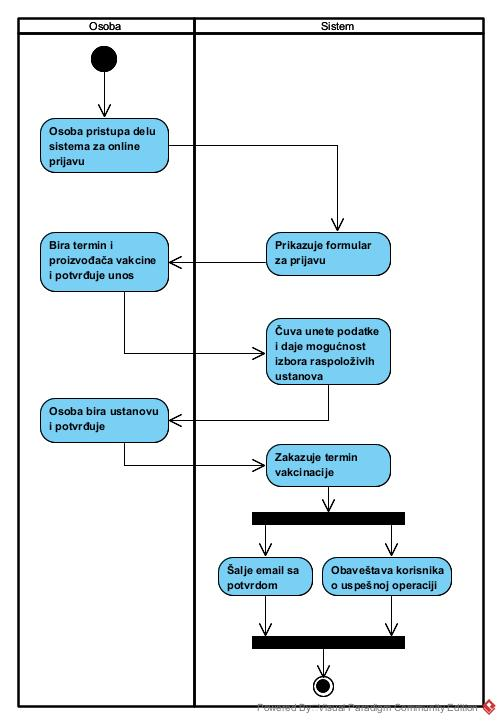
\includegraphics[scale=0.7]{Podnosenje_prijave_online}
\caption{Dijagram aktivnosti - Pondnošenje prijave online}
\end{figure}


\subsubsection{Slučaj upotrebe: Podnošenje prijave uživo}
%\subsubsection{Slučaj upotrebe: Evidentiranje prijave u sistemu}
\subsubsection{Slučaj upotrebe: Obaveštavanje o terminu vakcinacije online}
\subsubsection{Slučaj upotrebe: Obaveštavanje o terminu vakcinacije uživo}
\subsubsection{Slučaj upotrebe: Otkazivanje termina vakcinacije}
%\subsubsection{Slučaj upotrebe: Izadavanje online potvrde o vakcinaciji}
%\subsubsection{Slučaj upotrebe: Izdavanje uživo potvrde o vakcinaciji}


\subsection{Obaveštenje o drugoj/trećoj dozi vakcine}
\subsubsection{Slučaj upotrebe: ...}

\subsection{Informisanje}
\subsubsection{Slučaj upotrebe: Sprovođenje statistike}
\subsubsection{Slučaj upotrebe: Kol-centar}

\subsection{Kovid propusnice}

U ovom poglavlju se bavimo formalizacijom rada sa kovid propusnicama. U nastavku je opisan slučaj upotrebe podnošenja zahteva i izdavanja kovid propusnice.

\subsubsection{Slučaj upotrebe: Izdavanje kovid propusnice}

%Prvih 5 tacaka je obavezno, ostale nisu - navesti potrebne
%Ne bi bilo loše da, ako se dodaje neki dijagram, stoji opis uz njega i da se negde u tekstu onda reveriše na tu sliku

\begin{itemize}
    \item \textbf{Kratak opis:} Korisnik bira opciju za podnošenje zahteva za kovid propusnicu. Sistem proverava podatke, izdaje propusnicu i vraća odgovarajuću poruku.
    \item \textbf{Učesnici:}
        \begin{itemize}
            \item Korisnik - želi brzo da dobije kovid propusnicu uz minimalan broj koraka
        \end{itemize}
    \item \textbf{Preduslovi:} Sistem je aktivan. Korisnik je registrovan i ima pristup internetu.
    \item \textbf{Postuslovi:} Korisnik je dobio kovid propusnicu.
    \item \textbf{Osnovni tok:}
        \begin{enumerate}
            \item Korisnik otvara stranicu za prijavu.
            \item Sistem prikazuje formular za prijavu.
            \item Korisnik unosi odgovarajuće podatke.
            \item Korisnik potvrđuje unos.
            \item Sistem vrši validaciju podataka.
            \item Korisnik otvara stranicu za podnošenje zahteva za izdavanje propusnice.
            \item Sistem prikazuje tri moguće opcije:
                \begin{itemize}
                    \item Izdavanje propusnice na osnovu primljene vakcine.
                    \item Izdavanje propusnice na osnovu negativnog PCR ili antigenskog testa.
                    \item Izdavanje propusnice na osnovu preležanog virusa.
                \end{itemize}
            \item Korisnik bira jednu od ponuđenih opcija.
            \item Sistem proverava zadovoljenost uslova.
            \item Sistem korisniku šalje mejl sa kovid propusnicom.
            \item Sistem obaveštava korisnika da je operaciju uspešno izvršena i da je propusnica poslata.
        \end{enumerate}
     
    %Ako postoje, podtokove nazivati sa P1, P2, ...   
    %\item \textbf{Podtokovi:}    
    
    %Alternativne tokove nazivati sa A1, A2, ...
    \item \textbf{Alternativni tokovi:}
        \begin{itemize}
            \item[A1.] \textbf{Neuspešno prijavljivanje.} Ukoliko u koraku 5 osnovnog toka sistem naiđe na neispravne podatke, obaveštava korisnika i zahteva ponovni unos podataka. Proces se nastavlja u koraku 3 osnovnog toka.
            \item[A2.] \textbf{Uslovi za izdavanje nisu zadovoljeni.} Ukoliko u koraku 9 osnovnog toga sistem ustanovi da nisu zadovoljeni odgovarajući uslovi za izdavanje propusnice, obaveštava korisnika. Proces se završava.
        \end{itemize}
    
    %Ako postoje, specijalne zahteve navesti ovde
    %\item \textbf{Specijalni zahtevi:}
        
    \item \textbf{Dodatne informacije:}
        \begin{itemize}
            \item Podaci koji su potrebni za prijavu na sistem su korisničko ime i lozinka.
            \item Uslovi za izdavanje propusnice su:
                \begin{itemize}
                    \item Druga doza vakcine je primljena pre manje od 7 meseci ili  je primljena treća doza vakcine.
                    \item Postojanje negativnog PCR testa koji nije stariji od 72 sata ili antigenskog testa koji nije stariji od 48 sati.
                    \item Virus je preležan pre manje od 7 meseci.
                \end{itemize}
            \item Kovid propusnica sadrži QR kod na osnovu kog se proverava validnost propusnice.
        \end{itemize}
\end{itemize}

\subsubsection{Slučaj upotrebe: Validacija kovid propusnica}

\subsection{Testiranje}

\subsubsection{Slučaj upotrebe: Unos informacija o urađenom testu}

\end{document}
